\chapter{\label{chap:solution}Solution}

\textcolor{magenta}{Tentative solution length: between two to three pages, including the figures.}


%
%
%
\section{FC Implementation in AFCL}


\begin{figure}
  \centering
  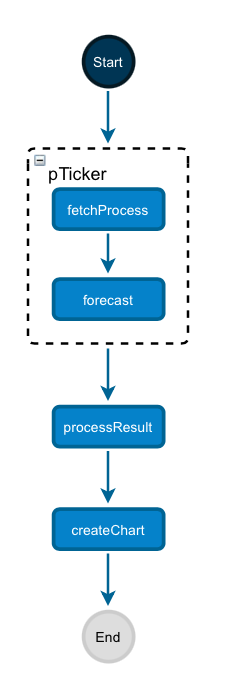
\includegraphics[height=12cm, keepaspectratio]{./assets/afcl}
  \caption{AFCL}
  \label{fig:afcl}
\end{figure}


Describe your FC (AFCL):
\begin{itemize}
    \item present a figure of your AFCL (you can use FC Editor)
    \item describe dataIns/outs inside the FC
    \item describe FC functions (function types)
    \begin{itemize}
        \item dataIns
        \item dataOuts
        \item purpose within the overall FC
    \end{itemize}
    \item explain compound functions
\end{itemize}

Discuss the FC complexity and the opportunities for distribution.



%
%
%
\section{Scheduler}

Our scheduler receives a AFCL YAML file as its input and in addition, the number of iterations and the concurrency limit.
As output, we directly create a YAML file as well.

For the implementation of our scheduler, we chose Rust. We created structs representing all the parts of the YAML and
used the \texttt{serde} library to serialise and deserialise them.

This way we can parse a full AFCL YAML file as input. Our program them loops through the \texttt{workflowBody} and
for each \texttt{parallelFor}, it applies the following algorithm:

\begin{itemize}
  \item Inputs: \texttt{iterations} and \texttt{concurrency\_limit}
  \item Variables: \texttt{concurrency\_limits} (\texttt{Map<String, usize>}), \\ \texttt{function\_iterations} (\texttt{Map<String, usize>}) and \\ \texttt{est} (\texttt{Map<String, (f64, f64)>})
  \item For \texttt{i} in \texttt{0...iterations}, loop through functions in \texttt{parallelFor} block:
    \begin{enumerate}
      \item Look up FDs in database and insert function names in all maps if not already contained
      \item Sort FDs by the start time stored in \texttt{est} and loop through them:
        \begin{enumerate}
          \item If FD has not yet reached the \texttt{concurrency\_limit} in \texttt{concurrency\_limits}, select it and update \texttt{concurrency\_limits}.
          \item Otherwise, reset the limit and increase the start time in \texttt{est}.
        \end{enumerate}
  \end{enumerate}
\end{itemize}

After running the algorithm, we know how to split a \texttt{parallelFor} into multiple \texttt{parallelFor}s and
create a new struct containing a \texttt{parallel} block with nested \texttt{parallelFor} blocks. The result is a
CFCL using the same structure, which means we can easily output it directly in YAML format.



%
%
%
\section{FC Implementation in CFCL}

\begin{figure}[h]
  \centering
  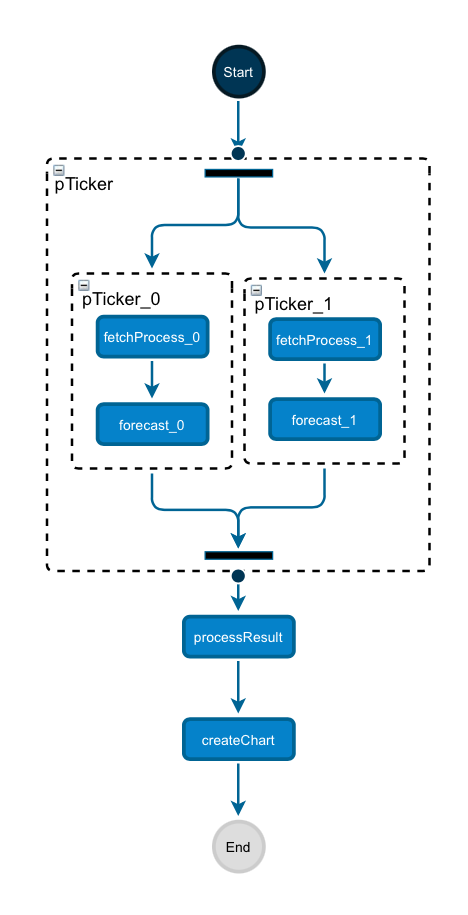
\includegraphics[height=12cm, keepaspectratio]{./assets/cfcl}
  \caption{CFCL}
  \label{fig:cfcl}
\end{figure}

As can be seen in \cref{fig:cfcl}, the single \texttt{parallelFor} from \cref{fig:afcl} has
been changed to a \texttt{parallel} section with two \texttt{parallelFor}s.

With 20 iterations and a concurrency limit of 2, 12 iterations of the \texttt{fetch\_prices\_js} and \texttt{forecast\_js}
functions were chosen for the first \texttt{parallelFor}. For the second \texttt{parallelFor},
8 iterations of the \texttt{fetch\_prices\_rs} and \texttt{forecast\_rs} functions were chosen.

% TODO: Discuss the CFCL complexity and expected theoretical speedup.



%
%
%
\section{Automatic Deployment}

For deployment, we used Terraform. We use it to deploy 8 functions to IBM cloud and
to create a bucket for use with AWS Forecast. Additionally, we created two Bash scripts
for compiling and packaging our Rust and TypeScript functions. We also use it to create
a \texttt{.env} which contains secrets and is used when compiling the functions.



%
%
%
\section{Fault tolerance}

\textcolor{magenta}{one paragraph}

If you use fault tolerance in your FC, describe which functions are monitored and which constructs are used.


%
%
%
\section{Helper tools from you}

Mention developed tools by you to help you to manage:
\begin{itemize}
    \item logs from \textit{xAFCL}
    \item parse AFCL and create CFCL
    \item parse AFCL and create CFCL
\end{itemize}
